\chapter{Project Outcome}

Assuming we are able to reach our goal by overcoming expected and unexpected challenges. 

\paragraph*{}
\textbf{Stage 1: Collaborative Localization and Mapping Using C-SLAM} \\
In the first stage, three robots are randomly placed within a room containing furniture and three distinct target objects. Each robot will independently scan the environment using LiDAR and Collaborative Simultaneous Localization and Mapping (C-SLAM) to determine its own position, identify the relative positions of other robots, and collaboratively create a shared map of the room. This process continues until the entire space is mapped. The use of C-SLAM is advantageous due to its decentralised nature, reducing the risk of a single point of failure and benefiting from mesh redundancy, allowing the task to continue if one robot fails. C-SLAM also enhances efficiency through lightweight communication, and though it requires more expensive sensors like LIDAR, this is offset by improved localization accuracy. Additionally, C-SLAM offers flexibility in environments with strong network connectivity and supports 3D mapping through the integration of depth cameras. This stage will be conducted at the ISE Lab.

\begin{figure}
    \centering
    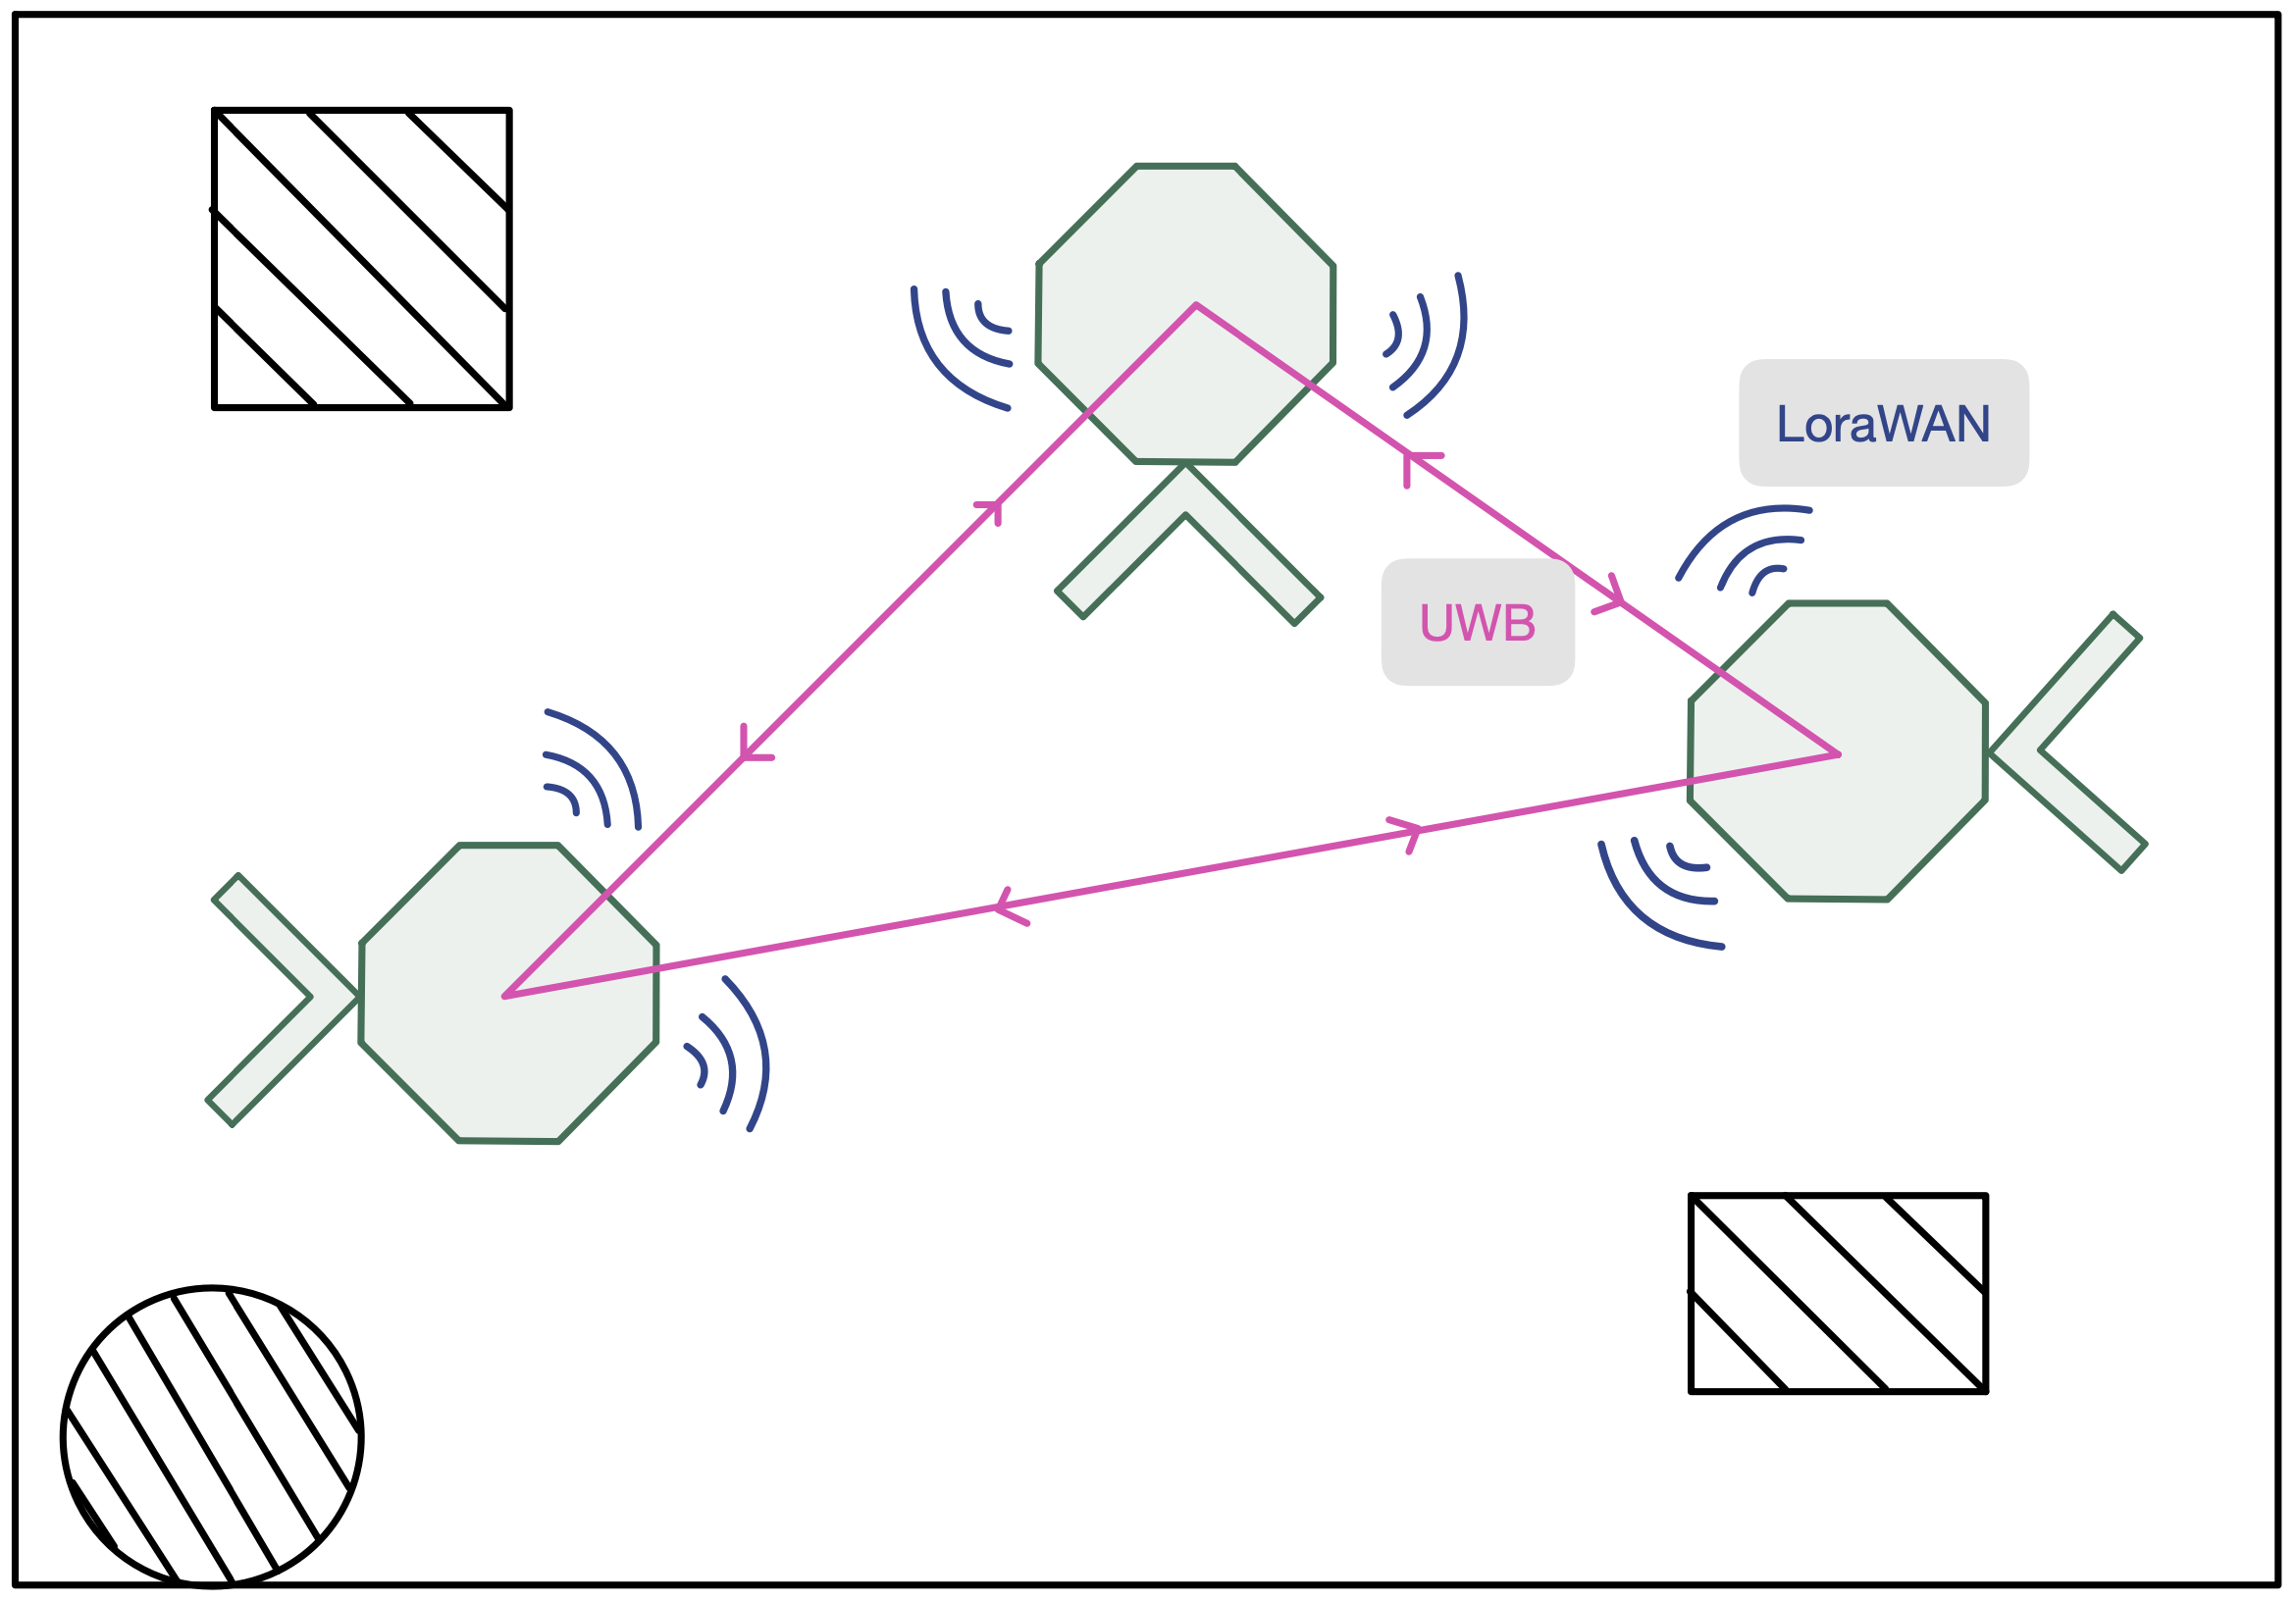
\includegraphics[width=0.5\linewidth]{assets/images/project_outcome/stage_1.png}
    \caption{Stage 1: 3 swarm robots(Green) localising and communicating with each other using LoraWAN and Ultra-Wide-Band UWB. the black objects are obstruction}
    \label{fig:phase1}
\end{figure}

\paragraph*{}
\textbf{Stage 2: Object Detection and Consensus for Identification} \\
After localization is complete, the swarm enters a standby state. When a named object is selected from the model database, the robots will collaborate to search for and identify the object. Upon locating it, the robot communicates the object’s position to the rest of the swarm. A consensus mechanism ensures that over 50\% of the robots agree that the correct object has been identified before any action is taken. The object, for testing purposes, is a static, slid-able geometric shape, such as a cube. The robots utilise RGB-D cameras for dynamic object detection, ensuring that movable items like pets or furniture are not unintentionally displaced. The depth data from the cameras enhances the robots’ 3D mapping capabilities and provides a cost-effective solution for object recognition.

\begin{figure}
    \centering
    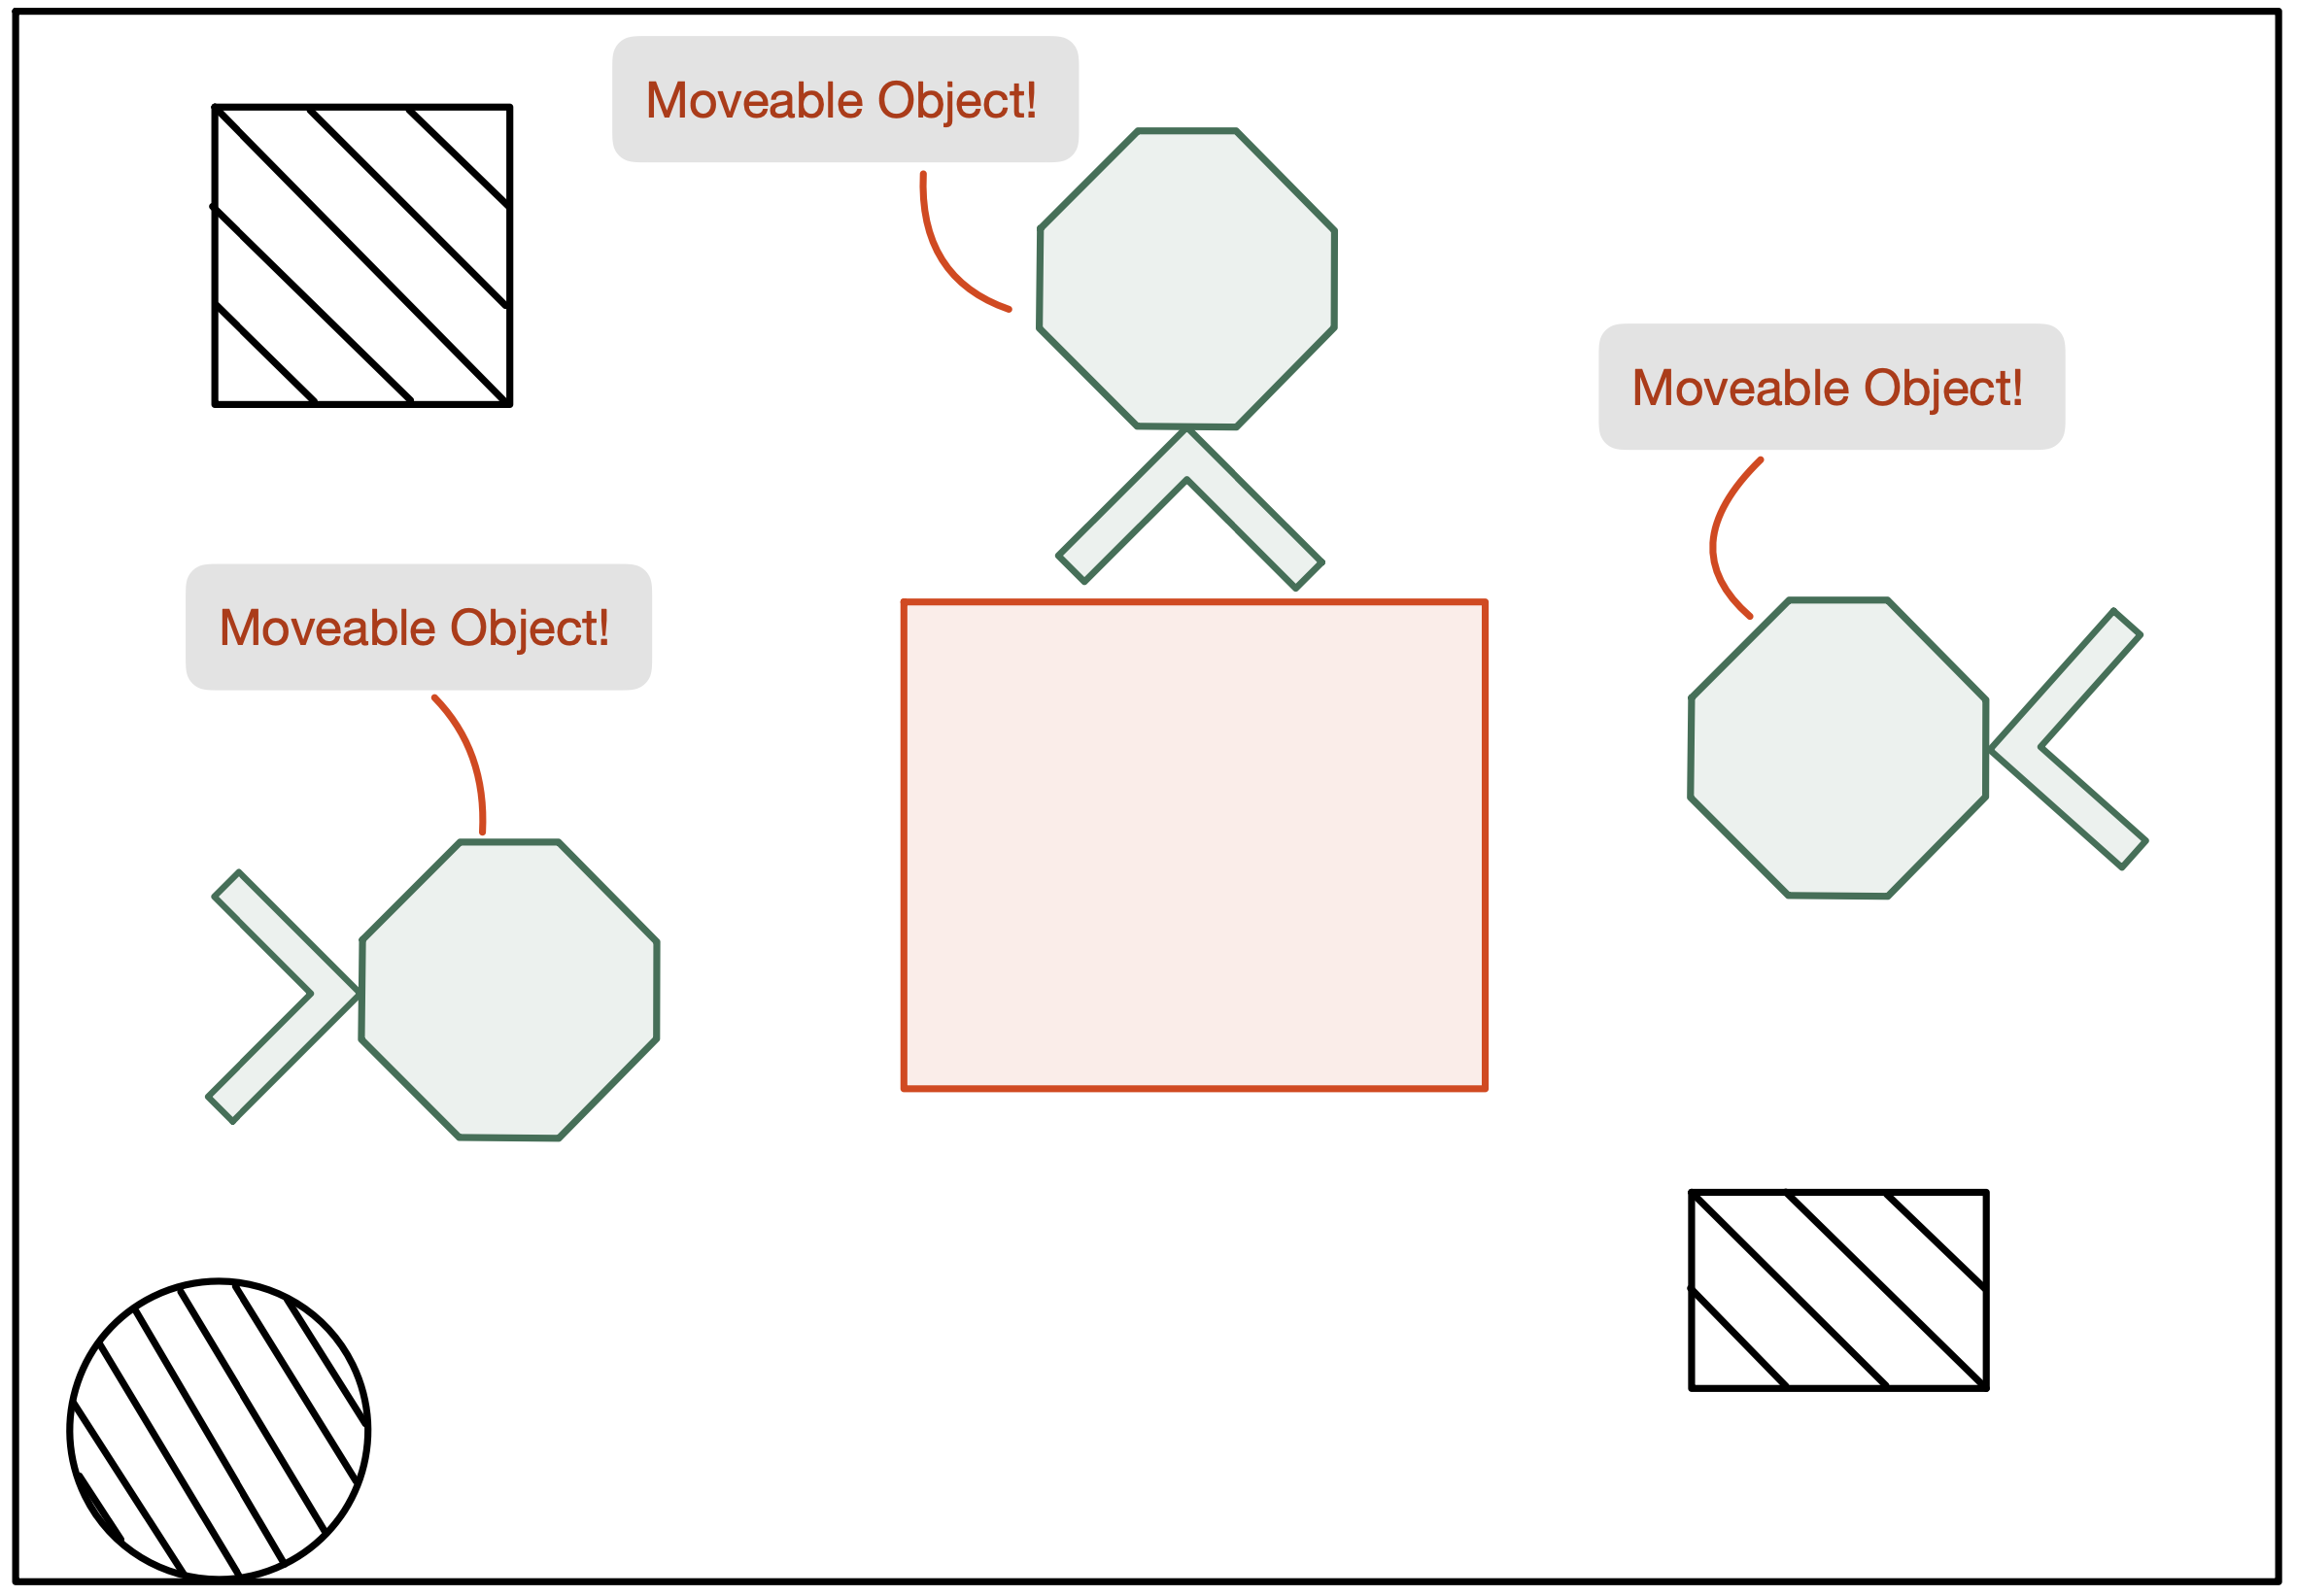
\includegraphics[width=0.5\linewidth]{assets/images/project_outcome/stage_2.png}
    \caption{Stage 2: A Red Object placed in the localised map, the robots detects the object using 2D/3D computer vision}
    \label{fig:phase2}
\end{figure}

\paragraph*{}
\textbf{Stage 3: Coordinated Object Movement} \\
Once consensus on the target object is reached, the robots will move towards it. Two robots, named Alpha and Beta, are assigned to secure the object along the X and Y axes at diagonal corners. A third robot, Gamma, provides the necessary force to push the object along a straight line toward its destination. The assignment of these roles is dynamic, with Alpha, Beta, and Gamma selected based on proximity to the object and destination. Alpha and Beta are assigned based on proximity to the object’s corners, while Gamma is the robot closest to the straight line between the object and destination. This method is both efficient and flexible, as role assignment occurs in real time, ensuring minimal delay. The destination is selected either by choosing the nearest edge of the object or by providing specific coordinates using the SLAM-generated map, allowing future integration with advanced interfaces like drag-and-drop UI.

\begin{figure}
    \centering
    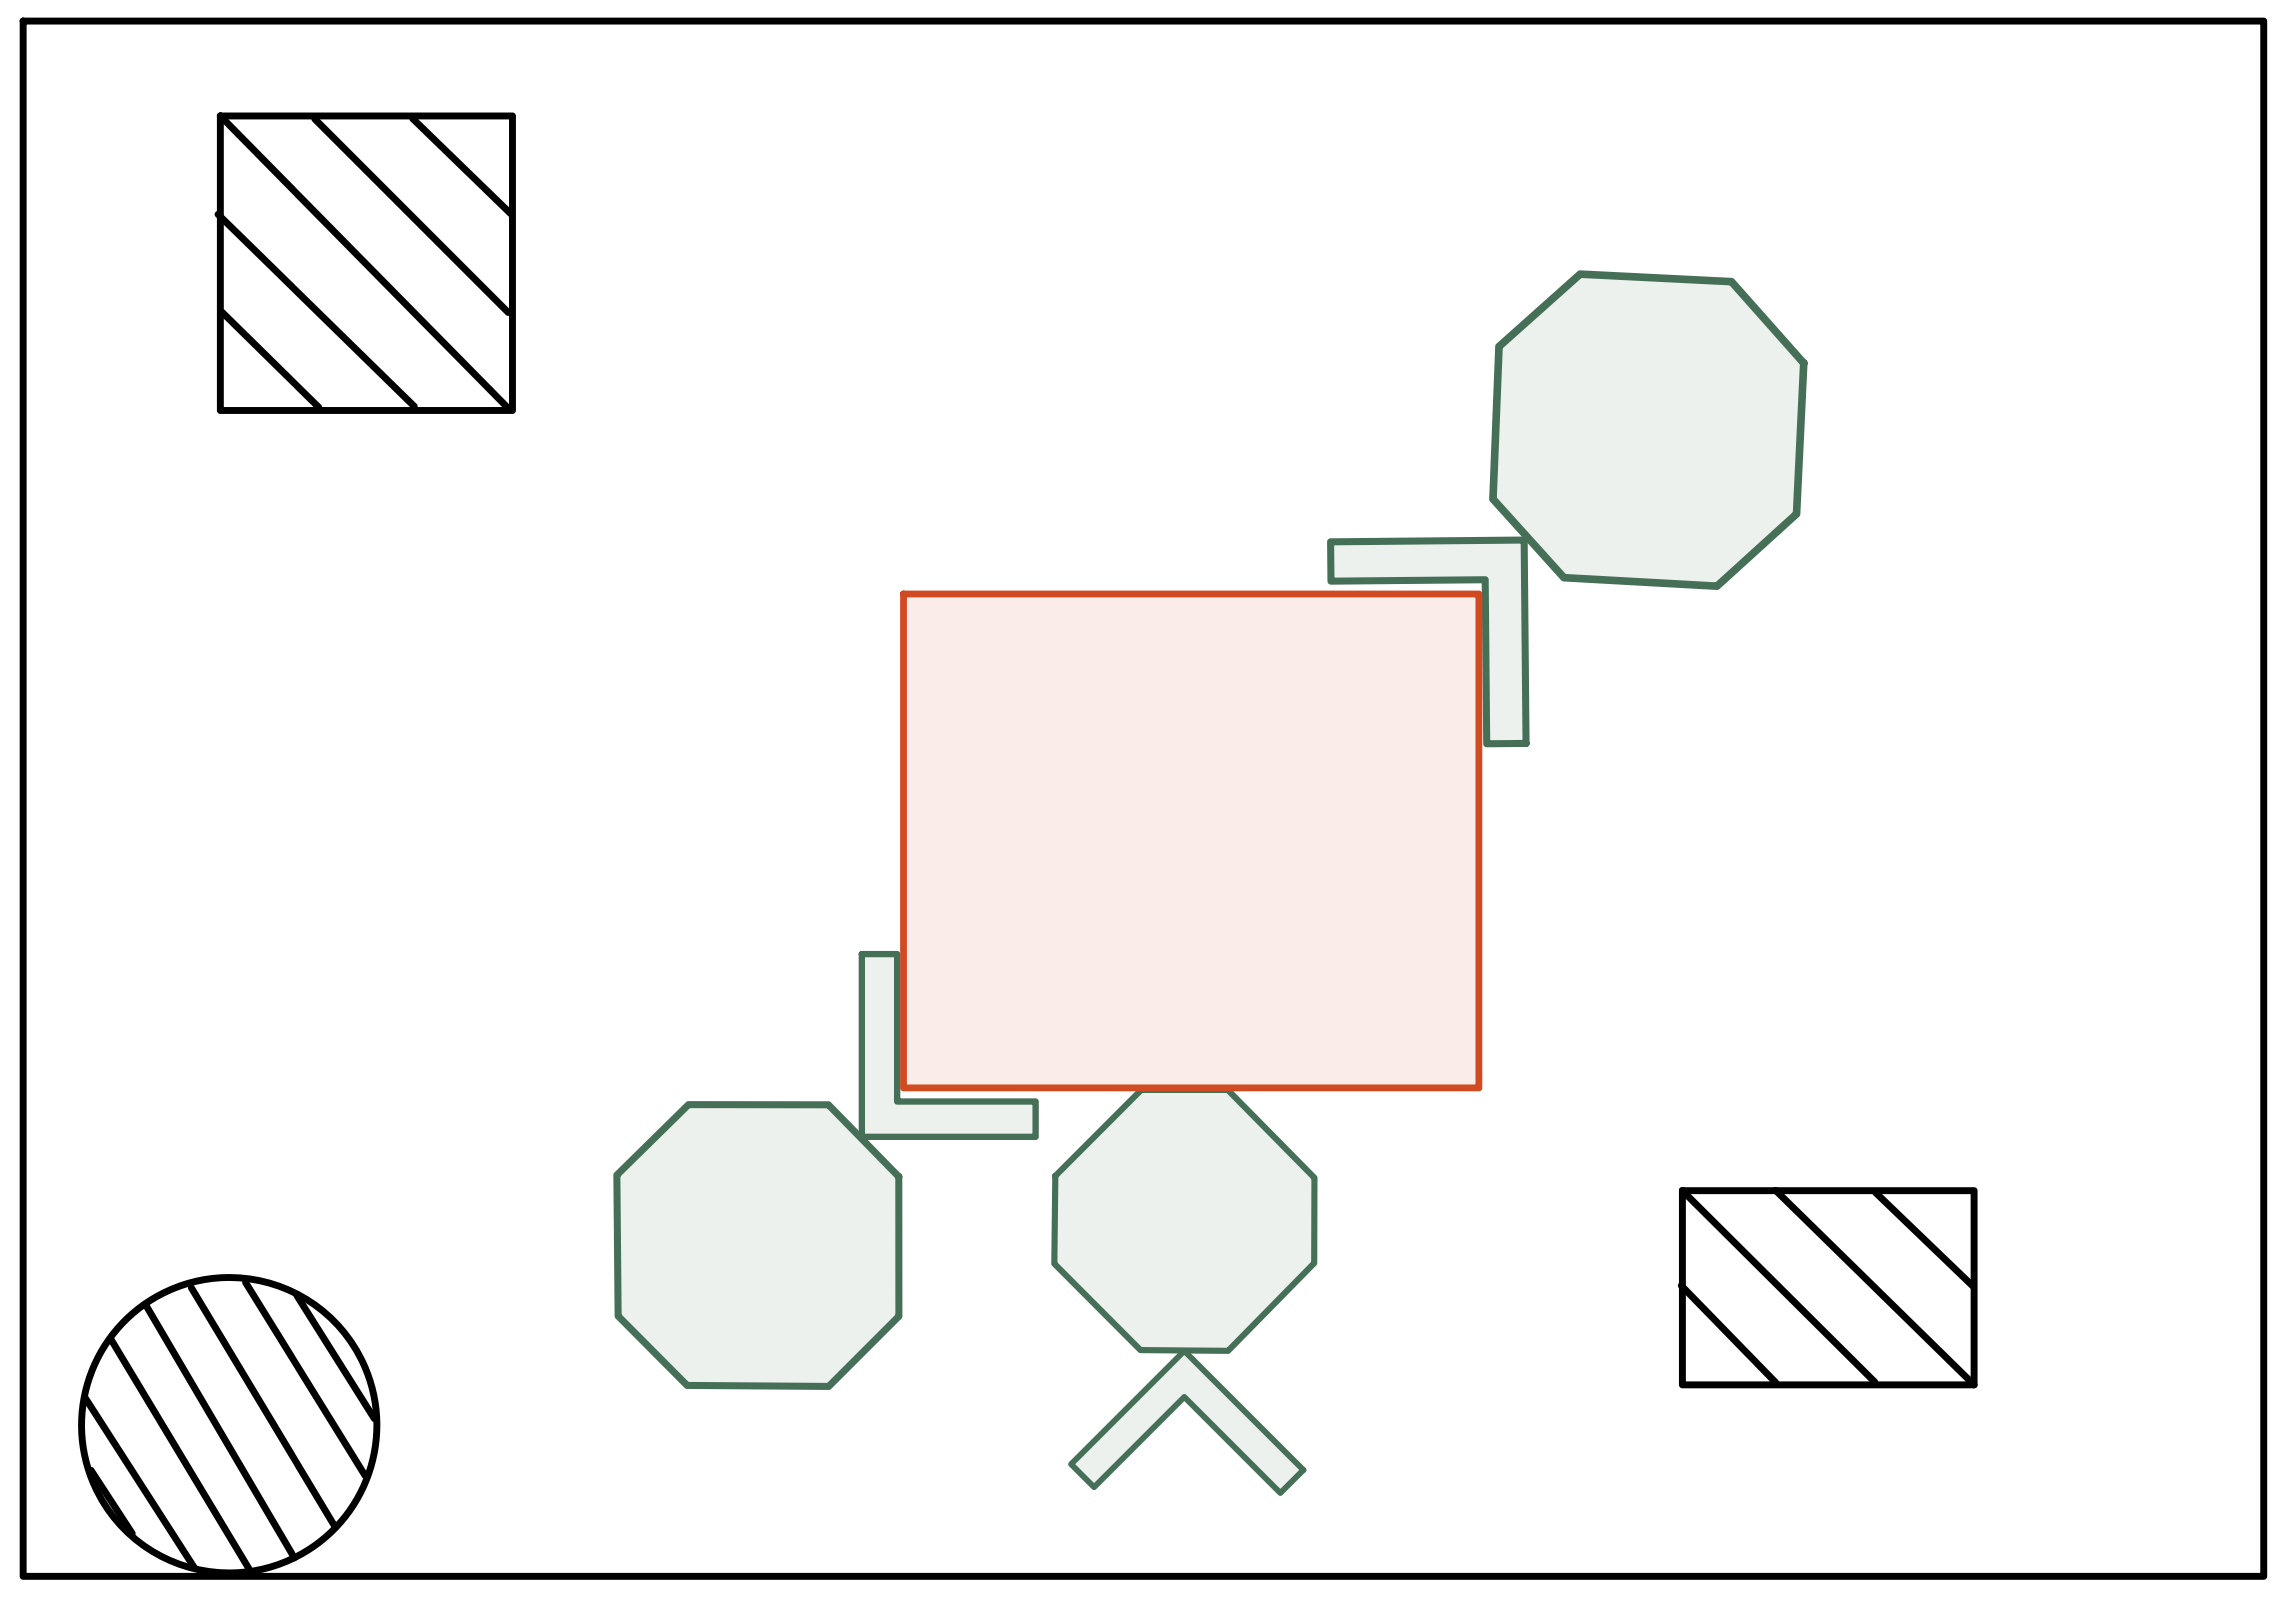
\includegraphics[width=0.5\linewidth]{assets/images/project_outcome/stage_3.png}
    \caption{Stage 3: The swarm moves and grip the object and ensure the object is securely in place}
    \label{fig:phase3}
\end{figure}

\paragraph*{}
\textbf{Stage 4: Object Movement and Environmental Constraints} \\
In the final stage, the robots push the object to the selected destination. To facilitate this, the object must have sufficiently low friction to allow sliding across the floor, as the team has chosen to restrict the object’s motion to two dimensions. The sliding method minimises potential challenges related to lifting or gripping the object

\begin{figure}
    \centering
    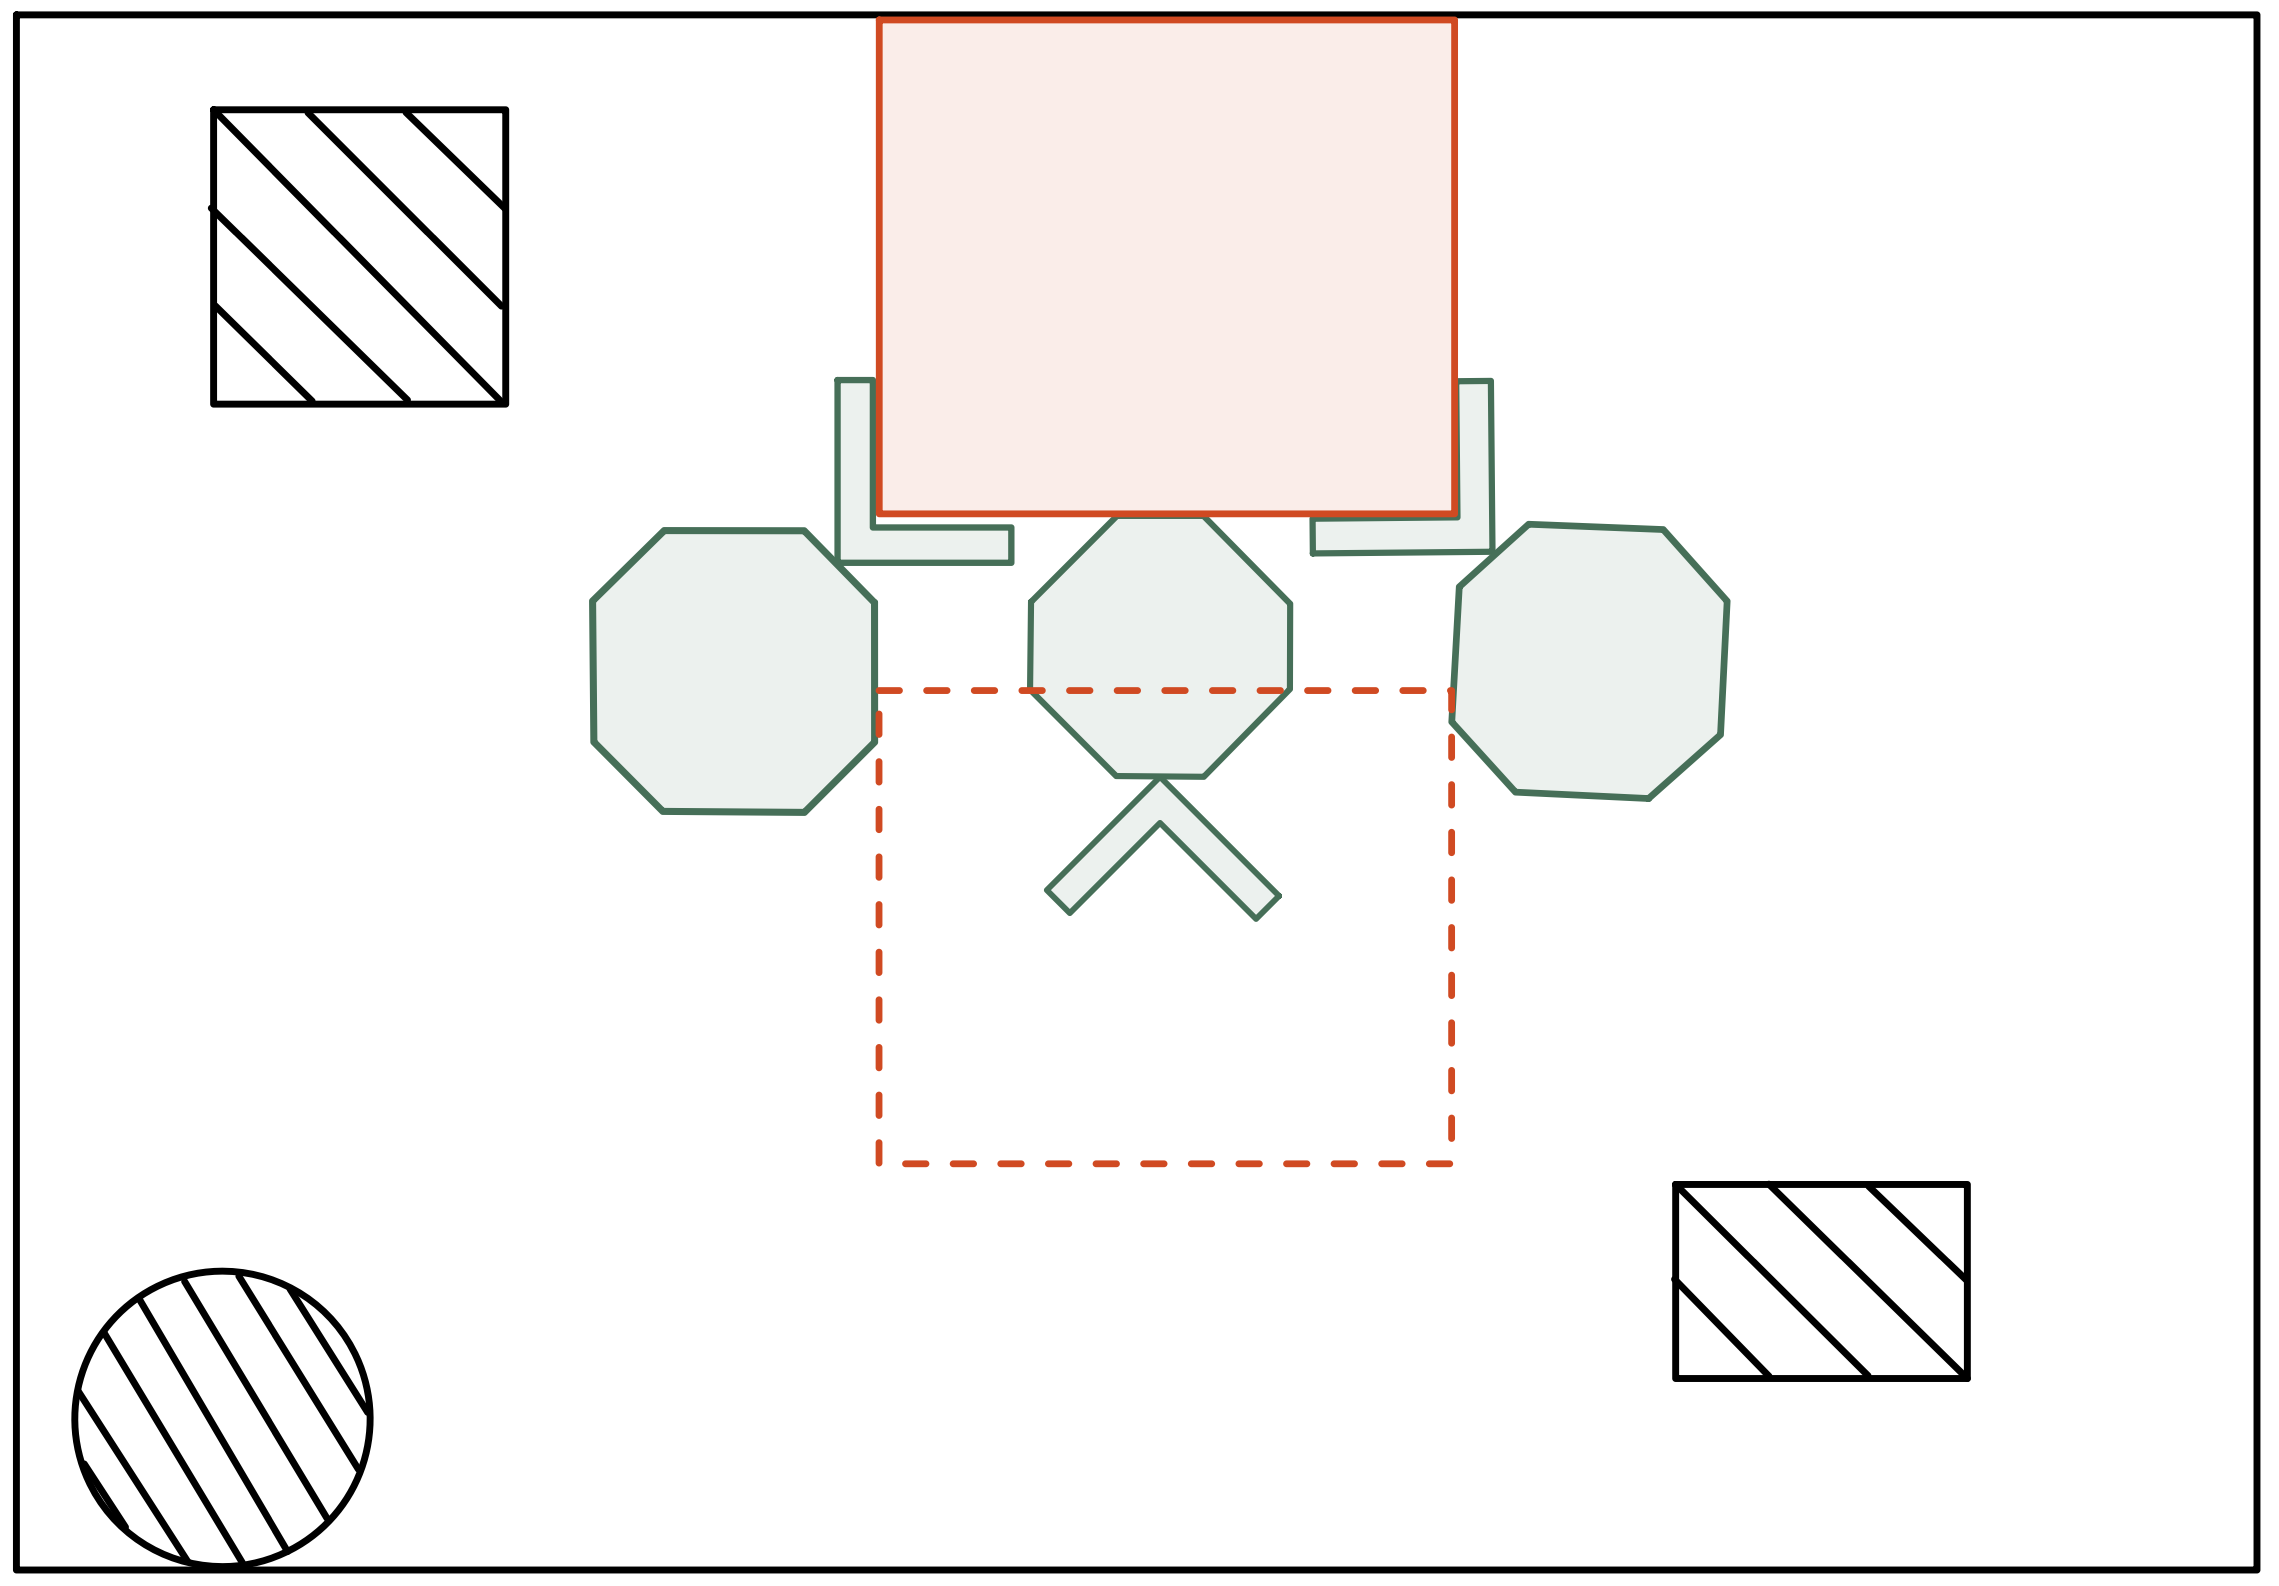
\includegraphics[width=0.5\linewidth]{assets/images/project_outcome/stage_4.png}
    \caption{Stage 4: The swarms then move the robot to the designated area and adjust the position of the robot dynamically}
    \label{fig:phase4}
\end{figure}
